%! TEX root = /Users/luigipertoldi/Tesi/tex/main.tex
\chapter{Theory Review}
\section*{The two-neutrino double-beta decay}
The two-neutrino double-beta decay ($2\nbb$) processes, first suggested by M.~Goeppert-Mayer in 1935 \cite{PhysRev.48.512}, can be schematically defined as:
\begin{equation*}
	\begin{split}
		\mathcal{N}(A,Z)\longrightarrow \mathcal{N}(A,Z+2)+2e^-+2\bar{\nu}_e \qquad [2\nu\beta^-\beta^-] \\
		\mathcal{N}(A,Z)\longrightarrow \mathcal{N}(A,Z-2)+2e^++2\nu_e \qquad [2\nu\beta^+\beta^+]\\
	\end{split}
\end{equation*}
where $\mathcal{N}(A,Z)$ represents a nucleus with mass number $A$ and atomic number $Z$. A $2\nu\beta^-\beta^-$ ($2\nu\beta^+\beta^+$) process consists of the simultaneous $\beta^-$ ($\beta^+$) decay of two neutrons (protons) in the same nucleus. The processes are generated at second-order in the perturbative expansion of weak interactions in the Standard Model.
\begin{figure}
	\centering
	\includestandalone{img/2nbbfey}
	\caption{Feynman graph for the two-neutrino double-beta decay.}
	\label{fig:2nbbfey}
\end{figure}

Since the $2\nbb$ decays have a four-body leptonic final state, the sum of the kinetic energies of the two decay electrons have a continuous spectrum from zero to the Q-value of the decay process (the recoil energy of the final nucleus is negligible), which is given by
\[Q_{\beta\beta}=M_i-M_f-2m_e\]
where $M_i$ and $M_f$ are, respectively, the masses of the initial and final nuclei (i.e. the energy levels of their ground states; if the transition occurs into an excited energy level of the final nucleus, $M_f$ must be replaced with the appropriate energy). 

A nucleus $\mathcal{N}(A,Z)$ can decay through a $2\nbb$ process if its ground state has an energy which is larger than the ground-state energy of the nucleus $\mathcal{N}(A,Z\pm2)$ plus twice the electron mass. Moreover, if a nucleus can decay through both the $\beta$ and $2\nbb$ processes, in practice the $2\nbb$ decay process is not observable, because its $\beta$ decay lifetime is much shorter than its $2\nbb$ decay lifetime (the half-life of $2\nbb$ is typically around $10^{19}-10^{24}$ yrs). Therefore, in practice the $2\nbb$ decay of a nucleus is observable only if its $\beta$ decay is energetically forbidden or strongly suppressed because of a large change of spin. The $\beta^-$ decay of a nucleus $\mathcal{N}(A,Z)$ is energetically forbidden if its ground-state energy is lower than the ground-state energy of the nucleus $\mathcal{N}(A,Z+1)$ plus the electron mass ($Q_{\beta^{-}}<0$). Typically, in $2\nu\beta^-\beta^-$ decays the energy levels of the three nuclei $\mathcal{N}(A,Z)$, $\mathcal{N}(A,Z+1)$, and $\mathcal{N}(A,Z+2)$ are of the type depicted in Fig.~\ref{fig:levelsGe76}, where the specific case of the \ce{^{76}Ge}, \ce{^{76}As}, and \ce{^{76}Se} nuclei is considered.
\begin{figure}[]
	\centering
	\subfigure
		{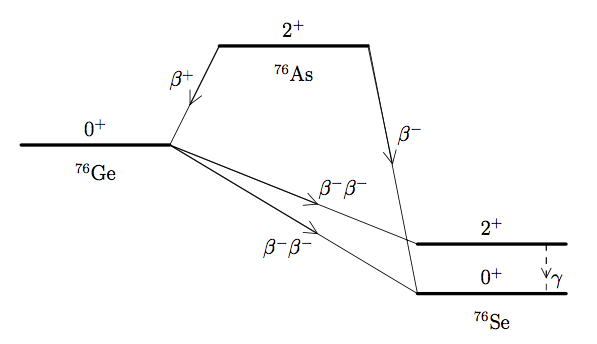
\includegraphics[width=5cm]{img/levelsGe76}}
	\subfigure
		{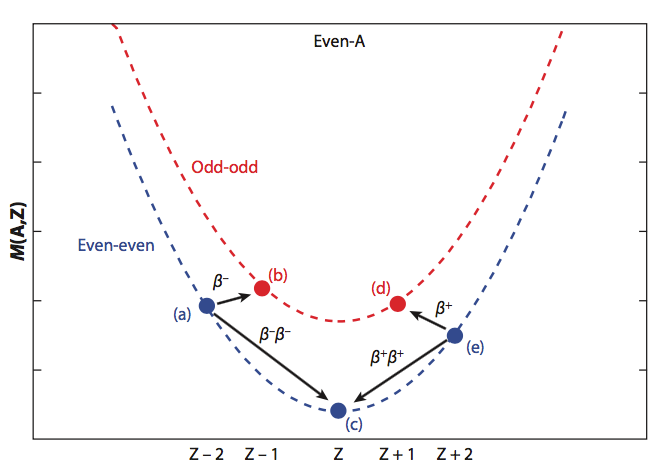
\includegraphics[width=5cm]{img/masspar}}
	\caption{Schematic illustration of the energy level structure of the $2\nu\beta^-\beta^-$ decay of \ce{^{76}Ge} into \ce{^{76}Se}.}
	\label{fig:levelsGe76}
\end{figure}

The naturally occurring isotopes which can decay through the $2\nu\beta^-\beta^-$ process, with forbidden or suppressed $\beta^-$ decay are 35, listed for example in \cite{Giunti:2007ry}. All of the initial and final nuclei in the $2\nu\beta^-\beta^-$ process are even-even, i.e. they have an even number of protons and neutrons. Their binding energy is larger than that of the intermediate odd-odd nuclei because of the pairing force acting between identical nucleons. For the same reason, all of the initial and final nuclei have a $0^+$ ground state. Therefore, all ground- state to ground-state transitions are $0^+\rightarrow0^+$. Ground-state transitions to an excited state of the final nucleus may be energetically allowed, as in the case of the $\ce{^{76}Ge}\rightarrow\ce{^{76}Se}$ $2\nu\beta^-\beta^-$ decay in Fig.~\ref{fig:levelsGe76}, in which there is an accessible $2^+$ excited state of \ce{^{76}Se}. However, due to a cancellation occurring in the phase space integral and the lower Q-value, the $0^+\rightarrow2^+$ double-beta decay is suppressed with respect to $0^+\rightarrow0^+$ \cite{Tomoda:1991}.

There are only six naturally occurring isotopes which can decay through the $2\nu\beta^+\beta^+$ process \cite{Haxton:1985am}. These isotopes have small Q-values and lifetimes which are much longer than the lifetimes of the $2\nu\beta^-\beta^-$. The reason for the rarity of $2\nu\beta^+\beta^+$-decaying isotopes and their small Q-values can be understood considering that that the decay $\mathcal{N}(A,Z)\rightarrow\mathcal{N}(A,Z-1)$ can occur either through the $\beta^+$ process $\mathcal{N}(A,Z)\rightarrow\mathcal{N}(A,Z-1)+e^++\nu_e$ or through the electron-capture process $e^-+\mathcal{N}(A,Z)\rightarrow\mathcal{N}(A,Z-1)+\nu_e$. Since $Q_{EC} = Q_{\beta^+}+2m_e$, the electron-capture process can occur even if the $\beta^+$ process is energetically forbidden ($Q_{\beta^+}<0$). Thus, in order have an energetically forbidden $\mathcal{N}(A,Z)\rightarrow\mathcal{N}(A,Z-1)$ transitions, the ground-state energy of $\mathcal{N}(A,Z)$ must be smaller than the ground-state energy of the nucleus $\mathcal{N}(A,Z-1)$ minus the electron mass ($Q_{EC}<0$). Considering as a reference energy the ground-state energy of the intermediate nucleus ($\mathcal{N}(A,Z+1)$ in $2\nu\beta^-\beta^-$ decays and $\mathcal{N}(A,Z-1)$ in $2\nu\beta^+\beta^+$ decays), the ground-state energy of the initial nucleus in a $2\nu\beta^+\beta^+$ decay must be at least $2m_e$ lower than in the case of a $2\nu\beta^-\beta^-$ decay. This implies that $2\nu\beta^+\beta^+$ decaying isotopes are more rare than $2\nu\beta^-\beta^-$-decaying isotopes. Moreover, for the same energy difference between the ground states of the intermediate and final nuclei, the energy difference between the ground states of the initial and final nucleus in a $2\nu\beta^+\beta^+$ decay is at least $2m_e$ lower than in the case of a $2\nu\beta^-\beta^-$ decay, leading to a correspondingly smaller Q-value. For these reasons, $2\nu\beta^+\beta^+$ decay has been less studied than $2\nu\beta^-\beta^-$ decay and in the following we will consider only $2\nu\beta^-\beta^-$ decays (we will simply refer to them with $2\nbb$). In any case, the neutrino properties of $2\nu\beta^+\beta^+$ decays are the same as those of $2\nu\beta^-\beta^-$ decays. Let us only mention that $\mathcal{N}(A,Z)\rightarrow\mathcal{N}(A,Z-2)$ transitions can occur not only through $2\nu\beta^+\beta^+$ processes, but also through the $EC\beta^+$ process $e^-+\mathcal{N}(A,Z)\rightarrow\mathcal{N}(A,Z-2)+e^++2\nu_e$ and the $2EC2\nu$ process $2e^-+\mathcal{N}(A,Z)\rightarrow\mathcal{N}(A,Z-2)+2\nu_e$.

The rate of $2\nbb$ can be calculated by invoking the recipe of the Fermi golden rule for simple $\beta$ decay. To a good approximation, the kinematic part (the phase space of the leptons emitted in the decay) and the nuclear part (the matrix element responsible for the transition probability between two nuclear states) can be factorized as
\[\Gamma^{2\nu}=G^{2\nu}(Q_{\beta\beta},Z)|\mathcal{M}^{2\nu}|^2\]
where $G^{2\nu}$ is obtained by integration over the phase space of four leptons emitted in the decay and can be calculated exactly. The nuclear matrix element $\mathcal{M}^{2\nu}$ deals with the nuclear structure of the transition and is much more difficult to evaluate. 

Denoting the 4-momentum of the two electrons and the two antineutrinos by $p^\alpha_i=(E_i,\mathbf{p}_i)$ and $q^\alpha_i=(\omega_i,\mathbf{q}_i)$, respectively ($i=1,2$), the relevant matrix element is given by
\[i\mathcal{M}=iG^2_FV^2_{ud}[\bar{u}(p_1)\gamma^\mu(1-\gamma_5)v(q_1)][\bar{u}(p_2)\gamma^\nu(1-\gamma_5)v(q_2)]J_{\mu\nu}-(p_1\leftrightarrow p_2)\]
The hadronic tensor $J_{\mu\nu}$ corresponds to the product of two nuclear currents written in the impulse approximation \cite{Tomoda:1991}. Including the implementation of the long-wave and closure approximation fot the hadronic tensor \cite{Tomoda:1991}, we obtain
\[\sum_\text{spin}|\mathcal{M}|^2=64G^4_F|V_{ud}|^4g^4_A(p_1\cdot p_2)(q_1\cdot q_2)|\mathcal{M}^{2\nu}|^2\;,\]
where the nuclear matrix element involves vector and axial couplings for Fermi and Gamow-Teller transitions in the form
\[g^2_A\mathcal{M}^{2\nu}=g^2_V\mathcal{M}^{2\nu}_F-g^2_A\mathcal{M}^{2\nu}_{GT}\;.\]

General methods for phase-space factor calculations in double-beta decay have been developed \cite{Doi:1981,Doi:1983,Tomoda:1991}. The phase-space factor is obtained by integration over all possible energies and angles of the leptons emitted in the decay. For the two-neutrino mode, these leptons are the two electrons and the two (anti)neutrinos:
\[G^{2\nu} \propto \int \text{d}^3p_1\text{d}^3p_2\text{d}^3q_1\text{d}^3q_2F(Z,E_1)F(Z,E_2)\delta(E_1+E_1+\omega_1+\omega_2-E_F-E_I)\;,\]
where $F(Z,E)$ is the Fermi function that describes the Coulomb effect on the outgoing electrons and $E_I$, $E_F$ are respectively the energies of the parent and the daughter nucleus.

In the Primakoff–Rosen approximation \cite{PrimakoffRosen} for the nonrelativistic Coulomb correction, the spectrum of the individual electrons can be analytically calculated:
\[\frac{d\Gamma}{dK}=\Lambda\cdot(K^5+10K^4+40K^3+60K^2+30K)(Q_{\beta\beta}-K)^5\;,\]
where $K$ is the sum of the kinetic energies of the two electrons in units of the electron mass. The overall constant factor is given by
\[\Lambda=\frac{G_F^4g_A^4|V_{ud}|^4F^2_\text{PR}(Z)m_e^{11}}{7200\pi^7}|\mathcal{M}^{2\nu}|^2\]
with $F_\text{PR}(Z)=2\pi\alpha/Z(\-e^{-2\pi\alpha Z})$.
\begin{figure}
	\centering
	\includestandalone{img/energyspectra}
	\caption{Energy spectra for different double-beta decay modes: in blue the two-neutrino mode, red the Lorentz violating mode, green the neutrinoless mode.}
	\label{fig:energyspectra}
\end{figure}

\section*{The neutrinoless double-beta decay}
	The neutrinoless double-beta decay processes ($0\nbb$) of the types
\begin{equation*}
	\begin{split}
		\mathcal{N}(A,Z)\longrightarrow \mathcal{N}(A,Z+2)+2e^- \qquad [0\nu\beta^-\beta^-] \\
		\mathcal{N}(A,Z)\longrightarrow \mathcal{N}(A,Z-2)+2e^+ \qquad [0\nu\beta^+\beta^+] \\
	\end{split}
\end{equation*}
which have been proposed by W.~H.~Furry in 1939 \cite{PhysRev.56.1184}, are forbidden in the minimal Standard Model, because the conservation of the total lepton number is violated by two units. Considering that today we know, from oscillations experiments, that neutrinos are instead massive particles, there are two ways to characterize them: they could be Dirac (as all the other fundamental particles) or Majorana particles. Being a Majorana particle, as first proposed by E.~Majorana \cite{Majorana1932}, means basically do not distinguish between particle and anti-particle. $0\nbb$ decays, in the standard interpretation, are possible if neutrinos are massive Majorana particles. In this case, a nucleus which can decay through a $2\nbb$ process can also decay through $0\nbb$ process, albeit with a different lifetime. Also the other double-beta decay modes mentioned above have their neutrinoless analog. However, as reviewed in \cite{Rodejohann:2011mu}, should be noted that there are many other well-motivated particle physics scenarios and frameworks that allow for $0\nbb$, treated as negligible contributions in the standard interpretation.

	Considerable experimental efforts are being dedicated to the detection of $0\nbb$, as such experiments represent the only practical way of establishing the nature of neutrino mass and therefore of shedding light on the mechanism of the tiny (but nonzero) neutrino mass generation established by neutrino oscillation experiments
